\documentclass{article}
\usepackage{tikz, comment}
\usepackage{pifont}
\usepackage{fontspec, pgfplots}
\usetikzlibrary{arrows, decorations.markings, decorations.pathreplacing}
\begin{comment}
:Title: Not defined yet
:Tags: cardioid;absolute value rules;focus of a parabola;parabola;inverse of a matrix, matrix inverse , multiplicative inverse of a matrix 
:Prob: 0.5614;0.538;0.52;0.5126;0.5091
:Author: Prof.Hu Ji-shan, HKUST
:Slug: No name yet

Description Here.........
\end{comment}
\begin{document}\centering 

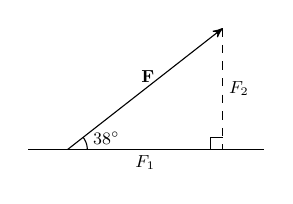
\begin{tikzpicture}[>=latex,xscale=.5*0.1, yscale=.5*0.1][font=\sf\small] 

%\draw[xstep=1cm,ystep=1cm,color=gray!80] (0, -1) grid (8, 8);

    	\foreach \x in {}
     		\draw (\x,2pt/2.5) -- (\x,-2pt/2.5)
			node[anchor=north] {\tiny$\x$}
			;

    	\foreach \x in {}
     		\draw (\x,2pt/1) -- (\x,-2pt/1)
			node[anchor=south] {\tiny$\x$}
			;
    	\foreach \y in {}
     		\draw (-2pt/1,\y) -- (2pt/1,\y)
			node[anchor=east] {\tiny $\y$}
			;

%\draw[->] (-10, 0) -- (50, 0)node[below] {$x$} ;
%\draw[->] (0, -0.5) -- (0, 2)node[left] {$y$} ;

\draw[] (-10, 0) -- (50, 0);

\draw[->, >=stealth'] (0, 0) -- (39.4, 30.8)node[black, left, midway, pos=0.6, xshift=0, yshift=0, scale=0.7]{${\bf F}$};

\draw[dashed] (39.4, 30.8)--(39.4, 0)node[black, right, midway, pos=0.5, xshift=0, yshift=0, scale=0.7]{$F_2$};

\node[below, scale=0.7] at ({39.4/2}, 0) {$F_1$};

\draw[black, samples=100, smooth, domain=0:38, variable=\t] 
		plot ({5*cos(\t)}, {5*sin(\t)}); 

\draw ({39.4-3}, 0)--++(0, 3)--++(3, 0); 

\node[xshift = 14, yshift = 4, scale=0.7] at (0, 0) {$38^\circ$};

\end{tikzpicture}
\end{document}